% Standalone vector figure extracted from manuscript.tex.
% Rebuild all figures from the project root: bash tkz/build.sh
\documentclass[tikz,border=2pt,class=IEEEtran]{standalone}
\usepackage{amsmath,amssymb,amsfonts}
\usepackage{xcolor}
\usetikzlibrary{positioning,arrows.meta,calc,backgrounds}

% Match the manuscript's IEEE Access text and math font settings.
\renewcommand{\textbf}[1]{{\fontseries{b}\selectfont #1}}
\renewcommand{\textit}[1]{{\itshape #1}}
\makeatletter
\AtBeginDocument{%
  \fontencoding{T1}\rmfamily\fontseries{m}\fontsize{10}{12}\selectfont
  \gdef\operator@encoding{T1}%
  \gdef\encodingdefault{T1}}
\makeatother

% ---- shared palette for review figures ----
\definecolor{cVLA}{HTML}{34618E}   % VLA lane / policy blue
\definecolor{cWM}{HTML}{9E4A3F}    % world-model lane
\definecolor{cCONV}{HTML}{5E4B8B}  % convergence purple
\definecolor{cGood}{HTML}{3A7D44}  % verified green
\definecolor{cWarn}{HTML}{B07A2A}  % caution amber
\definecolor{cPale}{HTML}{F2F0EA}  % pale panel fill
\tikzset{
  fnode/.style={draw=black!55, fill=white, rounded corners=1.5pt,
                inner sep=2.5pt, align=center, font=\fontsize{8}{9.5}\selectfont},
  flane/.style={draw=none, rounded corners=2pt, inner sep=3pt,
                align=center, font=\fontsize{8}{9.5}\selectfont\bfseries, text=white},
  farr/.style={-{Stealth[length=2mm]}, thick, black!60},
}


\newcommand{\figfont}{\fontsize{8}{9.5}\selectfont}

\begin{document}

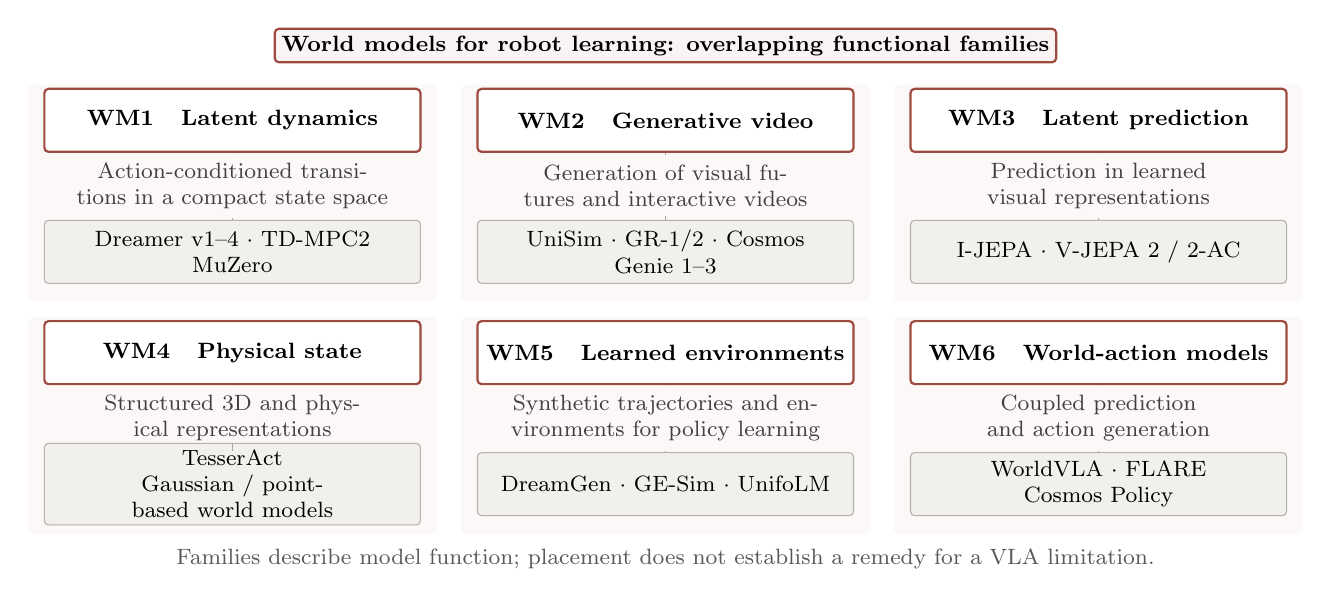
\begin{tikzpicture}[font=\figfont]
\node[fnode,draw=cWM,thick,fill=cWM!6,font=\figfont\bfseries] at (8.15,.5)
 {World models for robot learning: overlapping functional families};
\foreach \x/\y/\title/\function/\models in {
 2.65/0/{WM1\quad Latent dynamics}/{Action-conditioned transitions in a compact state space}/{Dreamer v1--4 $\cdot$ TD-MPC2\\MuZero},
 8.15/0/{WM2\quad Generative video}/{Generation of visual futures and interactive videos}/{UniSim $\cdot$ GR-1/2 $\cdot$ Cosmos\\Genie 1--3},
 13.65/0/{WM3\quad Latent prediction}/{Prediction in learned visual representations}/{I-JEPA $\cdot$ V-JEPA 2 / 2-AC},
 2.65/-2.95/{WM4\quad Physical state}/{Structured 3D and physical representations}/{TesserAct\\Gaussian / point-based world models},
 8.15/-2.95/{WM5\quad Learned environments}/{Synthetic trajectories and environments for policy learning}/{DreamGen $\cdot$ GE-Sim $\cdot$ UnifoLM},
 13.65/-2.95/{WM6\quad World-action models}/{Coupled prediction and action generation}/{WorldVLA $\cdot$ FLARE\\Cosmos Policy}}{
 \begin{scope}[shift={(\x,\y)}]
 \fill[cWM!4,rounded corners=2pt] (-2.6,-2.75) rectangle (2.6,0);
 \node[fnode,draw=cWM,thick,text width=46mm,minimum height=8mm,font=\figfont\bfseries] (h) at (0,-.45) {\title};
 \node[align=center,text width=46mm,text=black!75] (f) at (0,-1.28) {\function};
 \node[fnode,fill=cPale,draw=black!30,text width=46mm,minimum height=8mm] (m) at (0,-2.12) {\models};
 \draw[black!35] (h.south)--(f.north);
 \draw[black!35] (f.south)--(m.north);
 \end{scope}}
\node[text=black!65,align=center,text width=148mm] at (8.15,-6.02)
 {Families describe model function; placement does not establish a remedy for a VLA limitation.};
\end{tikzpicture}
\end{document}
